The fog grows thinner the further you climb. At the top of the ascent, you’re finally able to make sense of your surroundings--and the full extent of their destruction. The block's entire exterior wall has been torn away, along most of its roof and top floor. Rows of flagstone tiling end in a sheer cut overlooking a fog-choked riverside.\\

A breeze passes through the exposed mezzanine, producing a familiar whisking noise. It has likely been ages since you last heard it, but the sound is unmistakable: swaying branches. Venturing forth, you encounter a strange, pale species of tree that has taken root amongst the rubble. It stands at the height of two men, and bears no leaves or fruit. Its trunk sprouts from a man-height semi-circle of rubble; and you find that this heap was not merely the chance product of a crumbling ceiling. Its construction looks to have been purposeful, like the piled stones of bygone, primitive eras. Pacing around to its opening, you discover two dozen or so burnt corpses are nestled within. So that's where the block's prisoners ended up: as a macabre sort of potting material.\\

The branches quiver again, but this time there is no wind to brush them. Then the pale trunk unfurls, revealing something of a cross between a man and a dead tree. Its body pulses with a red glow, as if a hearth had been kindled within its gnarled belly. And when it lets out a scream, a jet of flame erupts from its jagged mouth.\\

\subsection*{Victory Condition}
Defeat Lukso the Metamorphosed

\subsection*{Doom Events}
\begin{itemize}
\item \textbf{Every 3rd Round:} \emph{Lukso screams, its body pulsing with a menacing glow.} For this Round, the \emph{Belch Fire} attack is replaced by \emph{Roaring Jet}.
\end{itemize}

\pagebreak

\subsection*{Encounter Table}
\begin{tcolorbox}
\textbf{Roll:} 2D6
\begin{center}
\begin{tabular}{ L | L | L }
\multicolumn{1}{c|}{\textbf{2}} & 
\multicolumn{1}{c|}{\textbf{3}} & 
\multicolumn{1}{c}{\textbf{4-5}} \\
\textbf{A:} \emph{Choke Slam}\newline \textbf{B:} \emph{Belch Fire} &
Move. \emph{Lunge} &
\textbf{A:} \emph{Belch Fire}\newline \textbf{B:} Move. Move \\
\hline
\multicolumn{1}{c|}{\textbf{6}} & 
\multicolumn{1}{c|}{\textbf{7}} & 
\multicolumn{1}{c}{\textbf{8}} \\
\textbf{A:} Move. \emph{Swipe}\newline \textbf{B:} \emph{Swipe. Lunge} &
\textbf{A:} \emph{Swipe. Lunge}\newline \textbf{B:} Move. \emph{Swipe} &
\textbf{A:} Move. \emph{Swipe}\newline \textbf{B:} \emph{Swipe. Lunge} \\
\hline
\multicolumn{1}{c|}{\textbf{9-10}} & 
\multicolumn{1}{c|}{\textbf{11}} & 
\multicolumn{1}{c}{\textbf{12}} \\
\textbf{A:} \emph{Belch Fire}\newline \textbf{B:} Move. Move &
Move. \emph{Lunge} &
\textbf{A:} \emph{Choke Slam}\newline \textbf{B:} \emph{Belch Fire}
\end{tabular}
\end{center}
\end{tcolorbox}

\subsection*{Enemy Sheet}
\hrule
\ \\
{\large \textbf{Lukso the Metamorphosed}}\\\\
\begin{tabular}{s s s}
\textbf{HP:} 24 & \textbf{Move:} 2\\
\textbf{P.DEF:} 1 & \textbf{F.DEF:} 2 \\
\end{tabular}\\

\emph{Hollow:} This entity ignores the Charmed, Maddened, and Fear conditions.\\

\emph{Sturdy:} This entity is immune to Knockback and Knockdown.\\

\emph{Bloodless:} This entity is immune to the Bleeding condition, and Poison, Toxic, and Bleed damage.\\

\textbf{Attacks:}
\begin{itemize}
\item \emph{Swipe} -  Deal 2 \emph{Unparryable} Slash damage to an adjacent entity.
\item \emph{Lunge} - Move 1. Deal 1 \emph{Unparryable} Crush damage and inflict Knockback 1 on an adjacent entity.
\item \emph{Choke Slam} - Deal 2 \emph{Unparryable} and \emph{Unblockable} Crush damage and inflict Knockdown on an adjacent entity.
\item \emph{Belch Fire} - Deal 2 Burn ranged damage to an entity that is within 3 tiles.
\item \emph{Roaring Jet} - Deal 2 \emph{Undodgeable} Burn ranged damage and inflict Blazing in a 3-hex cone centered on the target entity.
\end{itemize}
\hrule
\ \\

\pagebreak

\subsection*{Encounter Map}
\begin{center}
\framebox{
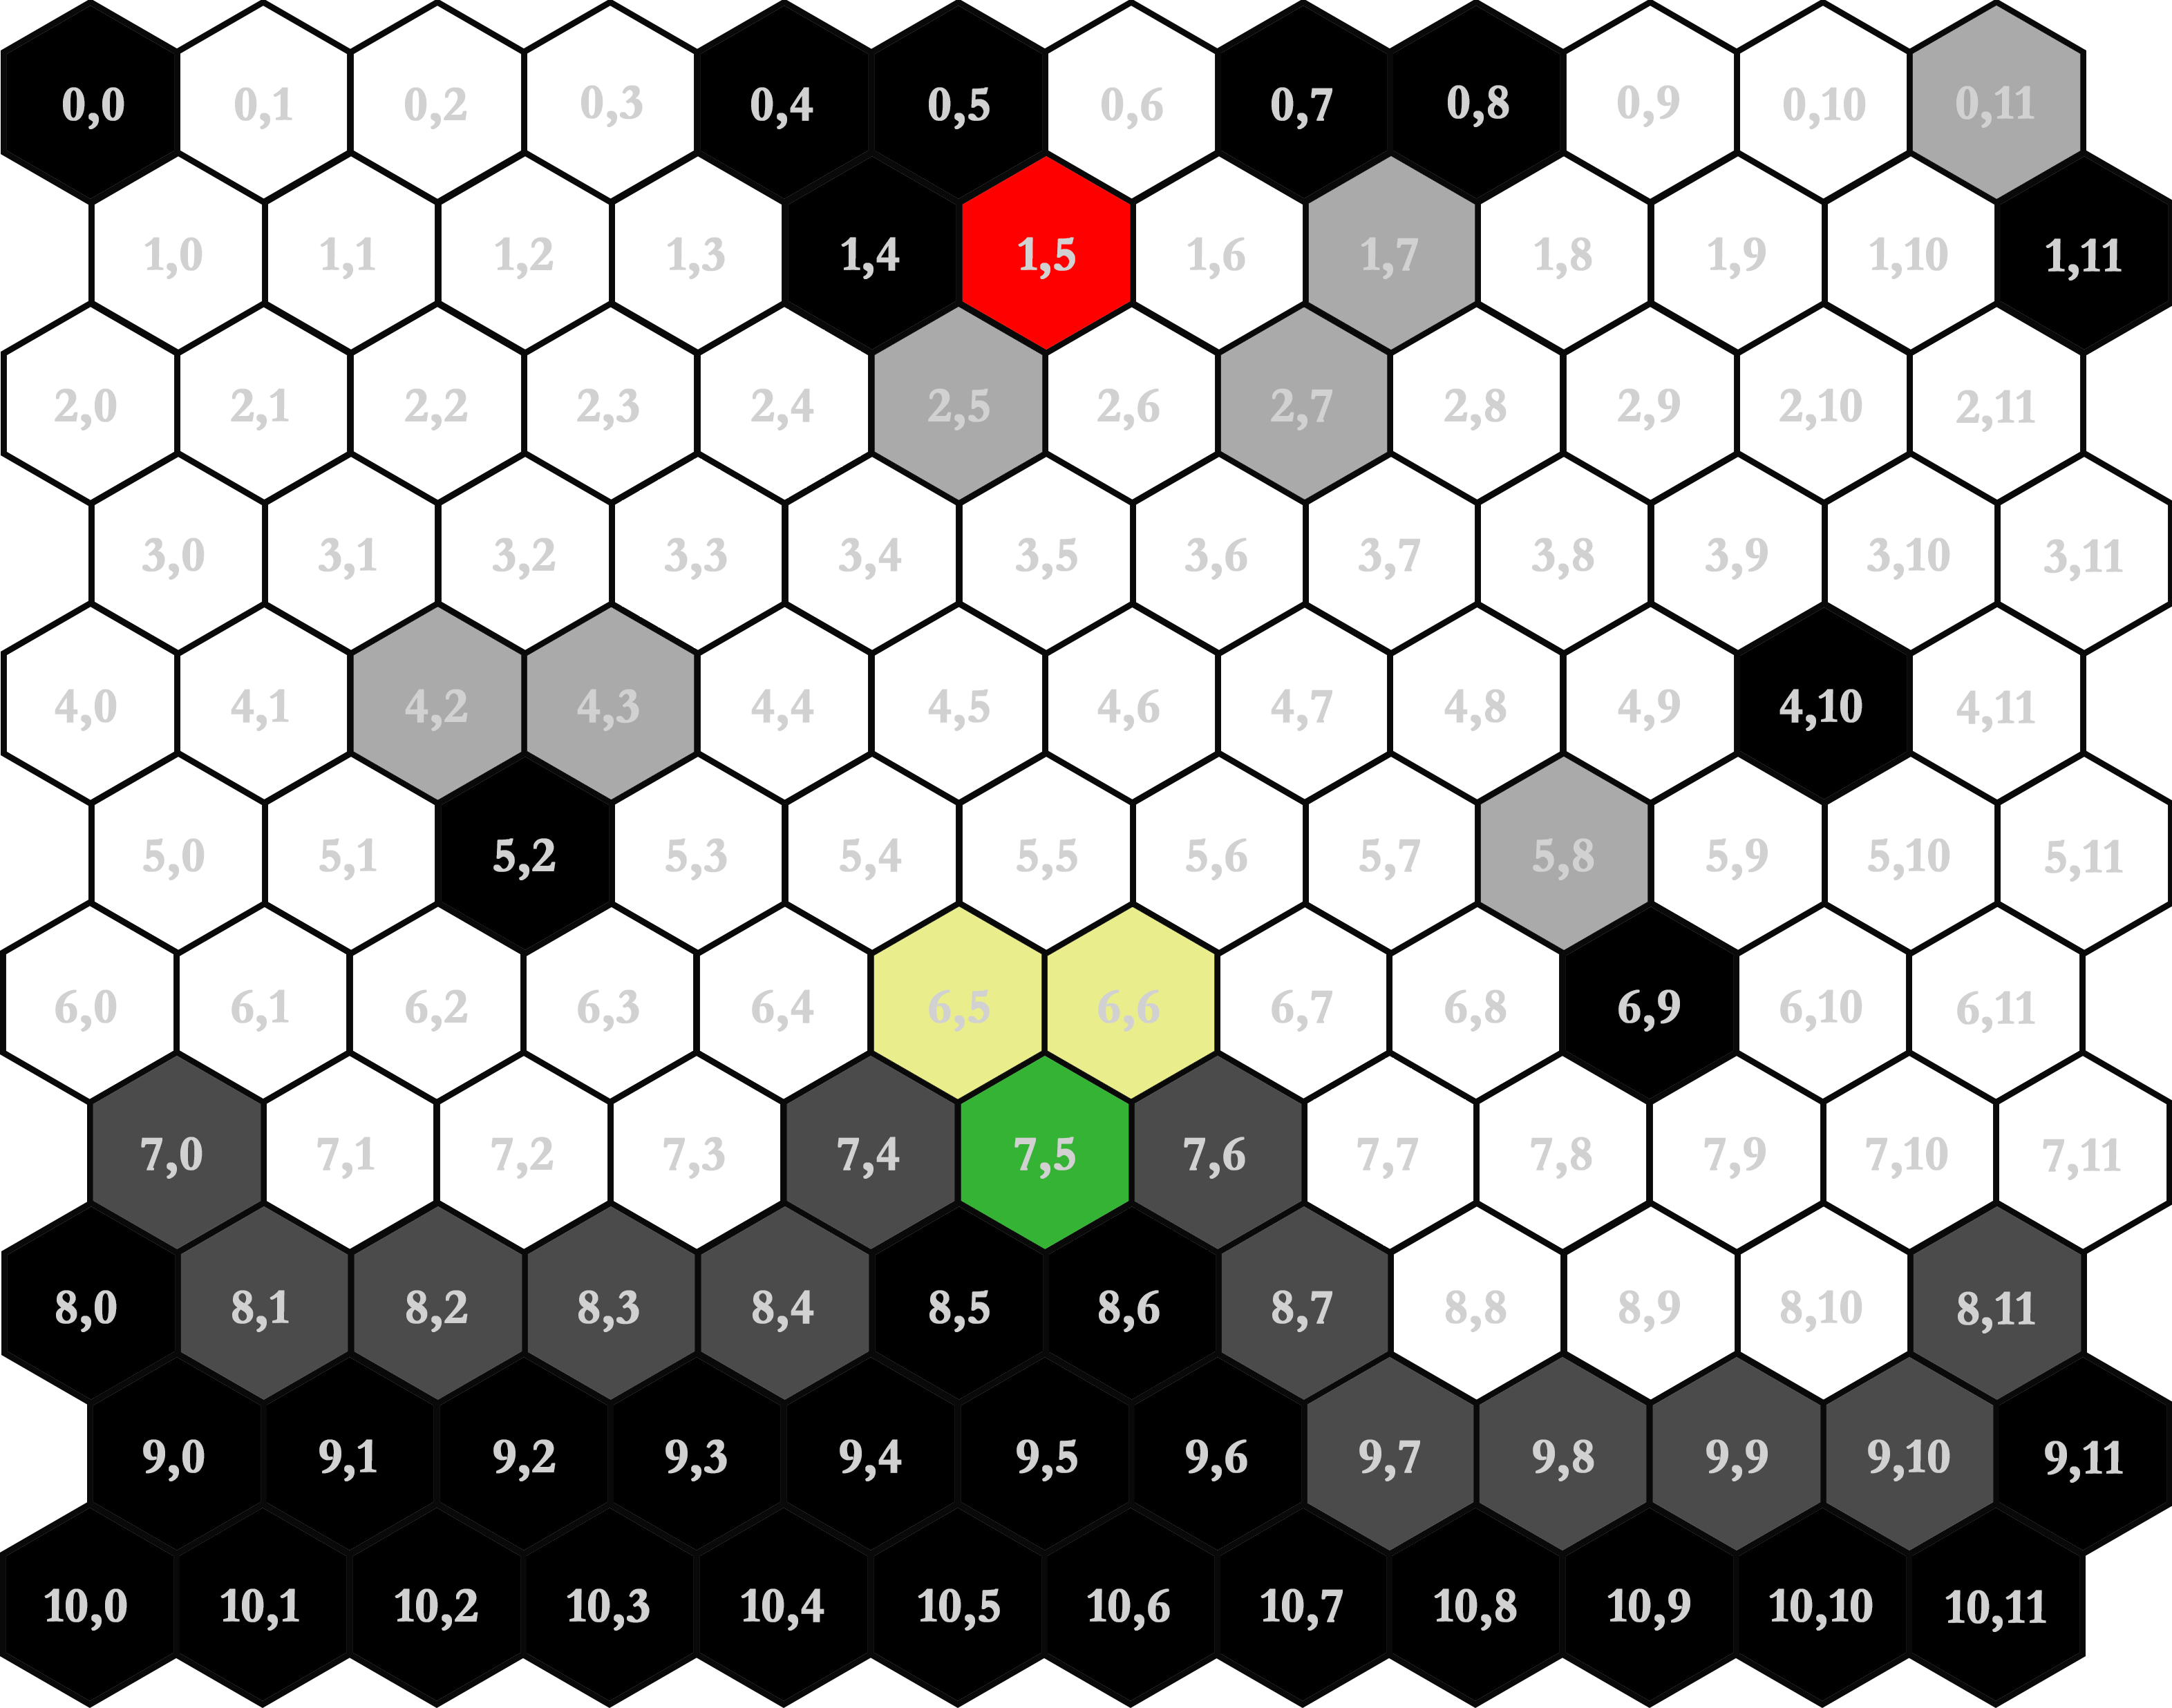
\includegraphics[width = 0.95\textwidth]{./maps/c315.png}
}
\end{center}

\subsection*{Setup Instructions}
\begin{itemize}
\item \textbf{Goldenrod:} Character Start Location.
\item \textbf{Red:} Enemy Start Location.
\item \textbf{Black:} Impassable Boundary/Full-Cover
\item \textbf{Dark Gray:} Pitfall. Any entity that enters this tile is defeated.
\item \textbf{Light Gray:} Half-Cover.
\item \textbf{Green:} Escape Tile.
\end{itemize}

\pagebreak

\subsection*{Victory}
The thing falls to its knees--or the closest anatomical feature that could be described as such. In a pose reminiscent of a drunkard’s morning-after, it issues a few wet coughs and then spews forth a stream of molten bile. After one last spurt, it collapses into the pool of its own steaming ichor. Its barklike skin sizzles and pops, giving off a rancid smell redolent of a tannery.\\

You have no word with which to describe the creature you’ve just slain. Your eyes likely never beheld such a thing, in this life or any other. But some of its features were... human in appearance, and disturbingly so.\\

>> Engorged Soul (30)\\
\gainx{Flamecast}\\
\notegain{c315a} Lukso is slain\\
>> \turnto{c316}

\subsection*{Defeat}

It's too late to do anything for the comrades of this cell block, but you resolve not to join them in that horrendous nest. The least you can do is survive.\\

You flee to the edge of the mezzanine, stopping just short and sending a shower of scree over its edge. But that thing is mere moments behind you, and so you throw yourself over just as a geyser of flame passes overhead.\\

At the bottom of the slope, you raise your head to discover a pulsing, red glow making its way down into the fog. You struggle to your feet, and limp across the yard. Given the size of your pursuer, you just need to make it to the security hallway. But each step is taken in agony, and you are haunted by the idea that its spindly arms might be just a hair’s breadth from your neck.\\

Eventually, you make it past the melted bars, and manage to drag yourself into the burnt contraband room before your grip on your consciousness fades.\\

When you awaken, the scorchmarks streaking across the walls take on a new and terrifying meaning.\\

>> Clear all \textbf{HP} slots\\
>> \textbf{HMN} - 1\\
>> \turnto{c35x1}

\subsection*{Retreat}

You take off running through the halls of the mezzanine, desperate for any hiding place or chance at escaping.\\

>> Clear all \textbf{HP} slots\\
>> \turnto{c324x1}